% !TEX ROOT = ../ersti.tex
\section{Informatik 100\%}

\begin{figure}[b]
\centering
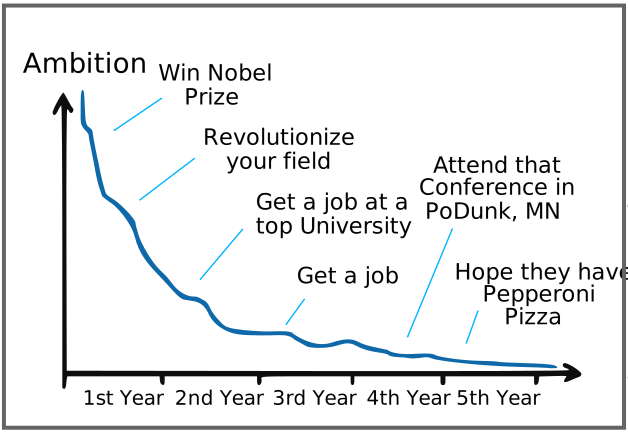
\includegraphics[height=5cm]{bilder/ambition.png}
\end{figure}

\begin{figure*}[th]
\centering
    \begin{subfigure}{.23\textwidth}
	    
\includegraphics[height=5cm]{bilder/backing_up_1.png}
    \end{subfigure}
    \begin{subfigure}{.23\textwidth}
	    
\includegraphics[height=5cm]{bilder/backing_up_2.png}
    \end{subfigure}
    \begin{subfigure}{.23\textwidth}
	    
\includegraphics[height=5cm]{bilder/backing_up_3.png}
    \end{subfigure}
    \begin{subfigure}{.23\textwidth}
	    
\includegraphics[height=5cm]{bilder/backing_up_4.png}
    \end{subfigure}
\end{figure*}

\subsection{Die ersten Semester}

Im ersten Semester hört ihr nach Studienverlaufsplan (s. Modulhandbuch) die \vl{Einführung in die Praktische Informatik} (\gls{IPI}), \vl{Einführung in die Technische Informatik} (\gls{ITI}), den \vl{Programmierkurs} (\gls{IPK}) und eine Mathematikvorlesung. Die \gls{IPI} vermittelt Grundkenntnisse und -konzepte der Informatik anhand mindestens einer Programmiersprache. Im \gls{IPK} vertieft ihr eure Programmierkenntnisse mit einer weiteren und in \gls{ITI} lernt ihr Grundlegendes über Rechnerarchitektur und die dazugehörigen logischen Schaltungen. Aufgepasst! Die \gls{IPI} ist in der Informatik eure einzige \emph{Orientierungsprüfung} und ihr müsst sie bis zum Ende des dritten Semesters bestanden haben.


\subsection{Später dann \dots{}}

\dots{} werden einzelne Themengebiete eröffnet und vertieft. Die Namen der Vorlesungen sprechen zum größten Teil für sich, zum Beispiel \vl{Datenbanken} (\gls{IDB1}) oder \vl{Betriebssysteme und Netzwerke} (\gls{BeNe} bzw. IBN). Außerdem besucht ihr ein \vl{Proseminar}, ein \vl{Seminar} sowie ein \vl{An\-fän\-ger--} und ein \vl{Fortgeschrittenen--Praktikum} (\gls{AP} und \gls{FP}). Diese unterscheiden sich von Vorlesungen, da von der Modulbeschreibung kein inhaltliches Thema vorgegeben wird, sondern lediglich die Veranstaltungsform.

\paragraph*{In Seminar und Proseminar} erklärt ihr jeweils den anderen Studis in einem Vortrag ein euch zuvor zugeteiltes Thema aus einem zusammenhängenden Themenbereich. Bei einem Proseminar wird dabei eher auf die Präsentation an sich geachtet, wobei es im Seminar normalerweise stärker auf den Inhalt ankommt. Das ist aber von der Lehrkraft abhängig und wird euch jeweils am Anfang erklärt.

\paragraph*{Praktika} sind i.d.R. Projekte mit einigermaßen freier Zeiteinteilung, die am Ende des Semesters fertig sein müssen und in Gruppen bearbeitet werden. Die Praktika wechseln von Zeit zu Zeit, es gibt aber üblicherweise jedes Jahr Angebote in Bereichen wie Technische Informatik und Software Engineering.

\subsection{Mathe und so \dots}

Informatikstudium in Heidelberg heißt, ihr hört vergleichsweise viel Mathe. Dabei habt ihr die Wahl zwischen mehreren Varianten, in der Hauptsache gibt es aber diese beiden Wege, bei denen ihr die für euer weiteres Studium relevanten Grundkenntnisse vermittelt bekommen sollt:

\begin{itemize}
	\item Mathe bei den Mathematikerinnen, also \vl{Lineare Algebra 1} (\gls{LA}) und \vl{Analysis 1} (\gls{Ana}). \gls{LA} und \gls{Ana} können entweder beide im ersten oder \gls{LA} im ersten und \gls{Ana} im dritten Semester gehört werden.
	\item \vl{Mathematik für Informatiker 1} (\gls{MafIn} bzw. IMI, entspricht etwa \gls{LA} 1) im ersten und \vl{Mathematik für Informatiker 2} (ersetzt \gls{Ana} 1) im zweiten Semester. Weiteres dazu im \autoref{mafin}.
\end{itemize}

Danach hört ihr \vl{Einführung in die Numerik} (\gls{Num0}) und eins der drei Module \vl{Analysis 2}, \vl{Mathematische Logik} oder \vl{Einführung in die Wahrscheinlichkeitstheorie und Statistik} (\gls{WTheo0}), sowie \emph{freiwillig} ein weiteres anrechenbares Mathemodul. Die Mathematikmodule unterscheiden sich stark von der Schulmathematik. Unterschätzt den Aufwand für die Vorlesungen nicht! Wollt ihr euer Informatikstudium mathematisch ausrichten (z.B. Richtung Wissenschaftliches Rechnen oder Machine Learning), empfehlen wir, die Mathevorlesungen \gls{LA} und \gls{Ana} bei den Mathematikerinnen zu hören.

\subsection{Programmieren. Und dann \dots}



Programmieren ist eine wichtige Fertigkeit, die ihr außerhalb von \gls{IPI} und \gls{IPK} hauptsächlich im Selbststudium erlernen oder vertiefen werdet. Solide Kenntnisse von unixoiden Systemen, wie Linux und OSX, sind immer Gold wert. Im Informatikstudium wird \emph{fast ausschließlich mit Linux} gearbeitet. Die Uni hilft aber auch noch ein bisschen: Neben den Pflichtkursen \gls{IPI} und \gls{IPK} gibt es in der \gls{Num0} praktische Übungen, in denen ebenfalls programmiert wird. Eigeninitiative ist aber dennoch wichtig, mit interessanten Projekten macht das aber auch enorm viel Spaß.


\subsection{Anwendungsgebiet}

Neben der wunderbaren Welt der Informatik sollt ihr euch aber auch mit deren Anwendungsgebieten auseinandersetzen. Dazu müsst ihr 24 \gls{LP} in mindestens einem anderen Fach erreichen. Entgegen der häufigen Vermutung hört ihr hier also einfach fachfremde Vorlesungen, um euren Horizont interdisziplinär zu erweitern, in denen ihr weder programmiert, noch sonstige Informatikkenntnisse vermittelt bekommt. Obwohl nur wenige Fächer im Modulhandbuch als Anwendungsgebiete vorgeschlagen werden, könnt ihr nach \emph{vorheriger} schriftlicher Bestätigung eures Prüfungssekretariats auch andere Fächer wählen, die euch interessieren. Dabei sind die Module von den Fachbereichen normalerweise fest vorgeschrieben, Nachfragen im Prüfungssekretariat des Anwendungsgebiets lohnt sich aber, da es manchmal doch einige Wahlmöglichkeiten gibt.


\subsection{Orientierungsprüfung}

Die \vl{Einführung in die Praktische Informatik} \emph{müsst} ihr, als eure Orientierungsprüfung, bis zum Ende des dritten Semesters bestanden haben.


\subsection{Prüfungen: wie und wieso?}

Um in den Vorlesungen \gls{LP} zu erhalten und somit das Modul abzuschließen, müsst ihr fast immer eine Klausur am Semesterende bestehen. Über die genauen Prüfungsmodalitäten informieren euch eure Dozierenden jeweils am Anfang des Semesters. Meist müsst ihr für die Klausurzulassung eine Mindestpunktzahl (i.d.R. 50\%) aus den Übungszetteln erreichen.

Häufig habt ihr pro Prüfung zwei Versuche, es ist also nicht so schlimm, wenn beim ersten Versuch nicht bestanden habt. Einige Dozierende weichen aber von der Standardregelung ab, teilen euch dies allerdings direkt am Anfang des Semesters mit. Informiert euch also am \emph{Anfang des Semesters} immer genau über die Bedingungen! Solltet ihr eine Prüfung auch beim Zweitversuch nicht bestehen, so besteht in bis zu vier Fällen die Möglichkeit, die Prüfung \emph{auf Antrag beim Prüfungsausschuss} ein weiteres Mal zu wiederholen (gilt nicht für Orientierungsprüfung und Bachelorarbeit). Besteht ihr auch diesen Versuch nicht, verliert ihr euren Prüfungsanspruch endgültig und werdet exmatrikuliert. Dies und weitere studienrelevante Vorschriften sind in der Prüfungsordnung geregelt, deshlab lohnt es sich definitiv, die Prüfungsordnung einmal komplett zu lesen. Außerdem kann sich diese leider immer mal wieder ändern, darauf sollte man achten.

\emph{Klausuranmeldungen sind immer verbindlich}. Überlegt euch also gut, ob ihr euch anmeldet. Solltet ihr euch sicher sein, die Klausur nicht zu bestehen, empfiehlt es sich, sich nicht anzumelden und die Vorlesung im nächsten Jahr noch einmal zu hören. Das Schöne an eurem Studiengang ist, dass die Noten der Grundpflichtmodule (\gls{IPI}, \gls{IPK}, \gls{ITI}, \gls{LA} 1 und \gls{Ana} 1 bzw. \gls{MafIn} 1 und 2) nicht in eure Abschlussnote zählen. Das heißt, dass auch wenn die ersten Semester mit der ganzen Mathematik vielleicht etwas hart sind, eure Abschlussnote darunter nicht unbedingt zu leiden hat.

\begin{figure}[t]
\centering

\includegraphics[width=.7\linewidth]{bilder/haskell.png}
\end{figure}

\begin{figure*}[b]
    
    \begin{subfigure}{.23\textwidth}
	    \includegraphics[height=5cm]{bilder/cant_sleep_1.png}
    \end{subfigure}
    \hfill
    \begin{subfigure}{.23\textwidth}
	    \includegraphics[height=5cm]{bilder/cant_sleep_2.png}
    \end{subfigure}
    \hfill
    \begin{subfigure}{.23\textwidth}
	    \includegraphics[height=5cm]{bilder/cant_sleep_3.png}
    \end{subfigure}
    \hfill
    \begin{subfigure}{.23\textwidth}
	    \includegraphics[height=5cm]{bilder/cant_sleep_4.png}
    \end{subfigure}

\end{figure*}

%\vspace{-\parskip}
